%\documentclass{article}

%%% NIPS DEFAULT PACKAGES
%\usepackage{nips_2017}
%\usepackage[utf8]{inputenc} % allow utf-8 input
%\usepackage[T1]{fontenc}    % use 8-bit T1 fonts
%%\usepackage{hyperref}       % hyperlinks
%\usepackage{url}            % simple URL typesetting
%\usepackage{booktabs}       % professional-quality tables
%\usepackage{amsfonts}       % blackboard math symbols
%\usepackage{nicefrac}       % compact symbols for 1/2, etc.
%\usepackage{microtype}      % microtypography

%%% RN stylefile
%\usepackage{morenotations,rotating}
%\usepackage{color,soul,upgreek}
%\usepackage{arydshln}
%\usepackage{wrapfig}
%\usepackage{soul}
%\usepackage{amsmath}
%\usepackage{empheq}
%\usepackage{mdframed,enumerate}


%\usepackage{xr-hyper}
%\externaldocument{nips18-coda-main}

%\usepackage{graphicx}
%\usepackage{caption}
%\usepackage{subcaption}

%%% Tikz Support
%\usepackage{tikz, pgfplots}
%\usetikzlibrary{intersections, calc, positioning, decorations.pathreplacing}
%\pgfplotsset{compat=1.8, xlabel style={anchor=west, align=center}, ylabel style={anchor=south, align=center}, samples=200, ymin=0, ymax=1, width=3cm, height=3cm, axis lines=middle, xticklabel style={/pgf/number format/.cd,frac,frac TeX=\frac}, yticklabel style={/pgf/number format/.cd,frac,frac TeX=\frac}, xtick=\empty,ytick=\empty, no markers, cycle list={{black,solid}}, samples=200}

%\newcommand{\amari}{}

%\title{\papertitle\\(\supplement)}
%%%Adversarial Learning Blurb
%%%How to \st{train} design your $f$-GANs

%%\author{RN}

%\begin{document}

%\maketitle

%\begin{abstract} %This is the supplement for paper "\papertitle".  %\end{abstract}

\addcontentsline{toc}{section}{Appendix}
%\part{Supplementary material on proofs and formal results}
\parttoc

%\section*{\supplement: table of contents}
%\noindent \textbf{Supplementary material on proofs and formal results}
%\hrulefill Pg \pageref{the_theo}\\
%\noindent Proof of Theorem \ref{thCODA1}\hrulefill Pg
  %\pageref{sec-proof-thCODA1}\\
%\noindent Proof of Lemma \ref{lemMU}\hrulefill Pg
  %\pageref{sec-proof-lemMU}\\
%\noindent Proof of Lemma \ref{lemHESS}\hrulefill Pg
  %\pageref{sec-proof-lemHESS}\\

%\noindent \textbf{Supplementary material on experiments} \hrulefill
%Pg \pageref{exp_expes}\\


\newpage

\section{Convexity of divergence}

\begin{theorem}\label{thCODA1}
For any $\A$, $\V$ such that $\A^\top \V \ve{1} = \ve{0}$, letting $D_{\exp}$ the Bregman divergence with generator
$\varphi^\star(z) \defeq \exp z$ and $\kl$ the generator for KL
divergence,
\begin{eqnarray}
 D_{\exp}(\V^\top
\ve{a}_i\|\clrlog({\ve{x}_i}))  & = &  q_i \cdot D_{\check{\kl}} (\ve{x}_i \|
\exp(\V^\top \ve{a}_i)) + r_i \cdot D_{g}(\ve{x}_i
\| \exp(\V^\top \ve{a}_i)), \forall i = 1, 2, ..., m\:\:,
\end{eqnarray}
with $q_i \defeq 1/g(\ve{x}_i)$ and $r_i \defeq q_i \cdot \sum_j
\exp\left(\ve{a}^\top_i
      \ve{v}_j\right)$, satisfying $r_i \geq d q_i$.
\end{theorem}
(Proof in \SM, Section \ref{sec-proof-thCODA1})

We can remark that
\begin{eqnarray}
\frac{1}{g(\ve{x}_i)} \cdot \sum_j
\exp\left(\ve{a}^\top_i
      \ve{v}_j\right) & = & \sum_j
\exp\left(\ve{a}^\top_i
      \ve{v}_j - x_{ij}\right) \check{x}_{ij}.
\end{eqnarray}

To generalize the notion of geometric average, consider any strictly convex function
$\varphi : \mathbb{R} \rightarrow \mathbb{R}$ at least three times
differentiable and with invertible derivative. Define the
$\varphi$-mean of $\ve{x}$ as
\begin{eqnarray}
\mu_{\varphi}(\ve{x}) & \defeq & \varphi'^{-1}\left(\E_i \varphi'(x_i)\right).
\end{eqnarray}
We now state a Lemma which will be essentially used for a particular
case of $\varphi$ but may be of independent interest for more general
cases, as explained in the following examples.
\begin{lemma}\label{lemMU}
Let $\varphi$ convex and at least three times differentiable. Let
\begin{eqnarray}
\phi(x) & \defeq & -\frac{\varphi'''(x)}{(\varphi''(x))^2}\:\:.
\end{eqnarray}
Then the $\varphi'$-mean $\mu_\varphi$ is convex (resp. concave) iff
\begin{eqnarray}
\phi(\mu_\varphi(\ve{x}))& \geq \mbox{ (resp. $\leq$)}& m \cdot \min_i
\phi(x_i) \:\:, \forall \ve{x}\:\:. \label{eqCONDNS}
\end{eqnarray}
\end{lemma}
(Proof in \SM, Section \ref{sec-proof-lemMU})
\begin{example}\label{exGEOM}
Take for example $F'(x) \defeq \ln x$ (geometric average). In this
case, $\phi(x) = +1$ and ineq. (\ref{eqCONDNS}) brings $1 \leq m$ for
the concavity of the mean and shows that $g$ is concave.
\end{example}
\begin{example}
Consider $F'(x) = -1/x$ (harmonic
average, over $\mathbb{R}_+$). In this case, $\phi(x) = + x$, so to prove the concavity of
the mean, we need to show $\mu_F(\ve{x}) \leq m \min_i x_i$, which is
equivalent to show
\begin{eqnarray}
\sum_i \frac{1}{x_i} & \geq & \max_i \frac{1}{x_i}\:\:,
\end{eqnarray}
and shows the concavity of the mean.
\end{example}
\begin{example}
Consider $F' = \exp$ (normalized
softmax). In this case, $\phi(x) = -\exp(-x)$, which shows that the
mean cannot be concave. To show its convexity, we need to show
equivalently
\begin{eqnarray}
\frac{1}{\sum_i \exp x_i} & \leq & \exp( - \max_i x_i)\:\:,
\end{eqnarray}
which is equivalent to $\sum_i \exp(x_i - \max_j x_j) \geq 1$, and
because of the non-negativity of the exponential,
shows the convexity of the mean.
\end{example}


\section{Proof of Theorem \ref{thCODA1}}\label{sec-proof-thCODA1}

First,
letting $\ve{y}_i \defeq \exp(\V^\top \ve{a}_i)$ for any $i = 1, 2, ...,
m$, and $\ve{v}_j$ the $j$-th row of $\V$ (as a column vector), we get
\begin{eqnarray}
\varphi^\star\left(\nabla\varphi(\veydagger_i)\right) & = & \sum_j
\exp\left( \log \left( \exp\left( \ve{a}^\top_i
      \ve{v}_j\right)\right)\right) = \sum_j
\exp\left(\ve{a}^\top_i
      \ve{v}_j\right)\label{eq1}.
\end{eqnarray}
We recall $g(\ve{x}) =
(\prod_k x_k)^{1/d}$, the geometric mean. So,
\begin{eqnarray}
g(\exp(\V^\top \ve{a}_i)) & = & \exp\left(\frac{1}{d} \sum_j \ve{a}^\top_i
      \ve{v}_j\right) = \exp((\A^\top \V \ve{1})_i) = \exp(0) = 1,
\end{eqnarray}
because of the constraint $\A^\top \V \ve{1} = \ve{0}_m$. Hence,
letting $\ve{y}_i \defeq \exp(\V^\top \ve{a}_i)$ for short, we obtain
$\check{\ve{y}}_i = \ve{y}_i$. Also, the dual symmetry of Bregman
divergences \citep{bnnBV} yields:
\begin{eqnarray}
D_{\exp}(\V^\top \ve{a}_i \|\clrlog({\ve{x}_i})) & = & D_{\kl} (\check{\ve{x}}_i \|
\exp(\V^\top \ve{a}_i))\:\:.
\end{eqnarray}
We now use Theorem \ref{th00}. It comes (letting again $\ve{y}_i \defeq \exp(\V^\top \ve{a}_i)$ for
short) that for any $i=1, 2, ..., m$,
\begin{align}
&g(\ve{x}_i) \cdot D_{\exp}(\V^\top \ve{a}_i\|\clrlog({\ve{x}_i}))\nonumber\\
=\;&   g(\ve{x}_i) \cdot D_{\kl} (\check{\ve{x}}_i \|
\exp(\V^\top \ve{a}_i))\nonumber\\
=\;&  D_{\check{\kl}}\left( \ve{x}_i \bigm\|
  \exp(\V^\top \ve{a}_i)\right) +
\varphi^\star\left(\nabla\varphi(\veydagger_i)\right) D_{g}(\ve{x}_i
\| \ve{y}_i)\nonumber\\
=\;&  D_{\check{\kl}}\left( \ve{x}_i \bigm\|
  \exp(\V^\top \ve{a}_i)\right) +
\left(\sum_j
\exp\left(\ve{a}^\top_i
      \ve{v}_j\right)\right)\cdot D_{g}(\ve{x}_i
\| \exp(\V^\top \ve{a}_i))\:\:,
\end{align}
which brings the statement of the Theorem. The fact that $r_i \geq d
q_i$ follows from the convexity of $\exp$.

\section{Proof of Lemma \ref{lemMU}}\label{sec-proof-lemMU}

Let $\mu_\varphi(\ve{x}) \defeq \varphi'^{-1}((1/m)\cdot \sum_i
\varphi'(x_i))$ the $\varphi'$-mean of the coordinates of
$\ve{x}$. Then
\begin{eqnarray}
\frac{\partial}{\partial x_i} \mu_\varphi(\ve{x}) & = &
\frac{1}{m}\cdot
\frac{\varphi''(x_i)}{\varphi''(\mu_\varphi(\ve{x}))}\:\:,\\
\frac{\partial^2}{\partial x_i \partial x_j} \mu_\varphi(\ve{x}) & = &
\frac{1}{m \varphi''(\mu_\varphi(\ve{x}))}\cdot \left(\delta_{ij}\cdot
  \varphi'''(x_i)-
  \frac{\varphi'''(\mu_\varphi(\ve{x}))}{m (\varphi''(\mu_\varphi(\ve{x})))^2}\cdot
  \varphi''(x_i) \varphi''(x_j)\right)
\end{eqnarray}
$\ve{x}$ being fixed, let $\tilde{\ve{y}}$ the vector defined by $\tilde{y}_i \defeq y_i
\cdot \varphi''(x_i)$ and let
\begin{eqnarray}
\phi(x) & \defeq & -\frac{\varphi'''(x)}{(\varphi''(x))^2}\:\:.
\end{eqnarray}
Let $\Phi$ the diagonal matrix with
$\Phi_{ii} \defeq \phi(x_i)$. The Hessian $\matrice{h}_{\mu_\varphi(\ve{x})}$ satisfies
\begin{eqnarray}
\ve{y}^\top \matrice{h}_{\mu_\varphi(\ve{x})} \ve{y} & = & \frac{1}{m
  \varphi''(\mu_\varphi(\ve{x}))}\cdot
\left(\frac{\phi(\mu_\varphi(\ve{x}))}{m}\cdot \tilde{\ve{y}}^\top
  \tilde{\ve{y}} - \tilde{\ve{y}}^\top
  \Phi \tilde{\ve{y}} \right)\nonumber\\
 & = & \frac{1}{m
  \varphi''(\mu_\varphi(\ve{x}))}\cdot
\tilde{\ve{y}}^\top \mathrm{Diag}\left(
  \frac{\phi(\mu_\varphi(\ve{x}))}{m}\cdot \ve{1} - \ve{\phi}(\ve{x})\right) \tilde{\ve{y}}
\end{eqnarray}
We see that when $\varphi''$ is
not zero everywhere, $\tilde{\ve{y}}$ spans the same set as $\ve{y}$,
so if $\varphi$ is convex, $\mu_\varphi$ is
convex iff
$(\phi(\mu_\varphi(\ve{x}))/m)\cdot \ve{1} - \ve{\phi}(\ve{x})
\geq \ve{0}$, that is
\begin{eqnarray}
\phi(\mu_\varphi(\ve{x}))& \geq & m \cdot \phi(x_i)\:\:, \forall i\:\:,
\end{eqnarray}
which is equivalent to the Lemma's statement.

%\section{Proof of Theorem \ref{thmSMOOTH}}
%We extend the definition of the geometric mean to $\Se\cup\partial\Se$ so that
%$g(\ve{x})=\prod_{j:x_j>0} x_j^{1/d^+}$, where
%$d^+=\vert\{j\,:\,x_j>0\}\vert$. In this way $\check{\ve{x}}$ is defined
%as a continuous function on the whole manifold with boundary. This is only a
%technical treatment as we assume $\ve{x}$ is given.

%By noting that $\exp(\clrlog(\ve{x}))=\check{\ve{x}}$, we have
%\begin{align}
%D_{\exp}(\ve{y}\,\Vert\,\clrlog(\ve{x}))
%&=
%\bm{1}^\top\bigg[ \exp(\ve{y}) - \check{\ve{x}} - \check{\ve{x}}\circ\left(\ve{y}-\clrlog(\ve{x})\right) \bigg]\nonumber\\
%&=
%\bm{1}^\top\exp(\ve{y}) - \check{\ve{x}}^\top \ve{y} +
%\mathrm{constant}\nonumber\\
%&=
%\sum_j \exp(y_j) - \sum_{j:x_j>0} \check{x}_j^\top y_j +
%\mathrm{constant}
%\end{align}
%Note that the coordinate cart $(y_1,y_2,\cdots)$
%only covers the interior of the plane $\ve{1}^\top\ve{y}=0$
%but cannot cover its boundary.
%On the boundary (where $y_j=-\infty$) we have to change the chart to $z_j=\exp(y_j)$.
%In this case the function becomes 
%\begin{align}
%D_{\exp}(\ve{y}\,\Vert\,\clrlog(\ve{x}))
%=\sum_j z_j - \sum_{j:x_j>0} \check{x}_j^\top \log{z}_j,
%\end{align}
%which is a smooth function near the boundary when $z_j=0$ and $x_j=0$.

\section{Proof of Lemma \ref{lemHESS}}\label{sec-proof-lemHESS}

We have
\begin{eqnarray}
\check{\kl}(\ve{x}) & = & \left(\sum_i x_i\log x_i - x_i\right) - \frac{1}{d}
\cdot \sum_{ij} x_i \log x_j
\:\:,\\
\frac{\partial}{\partial x_i} \check{\kl}(\ve{x}) & = & \log x_i -
\frac{1}{d} \cdot \sum_j \log x_j -\frac{1}{d x_i} \cdot \sum_j x_j
\\
 & = & -\frac{1}{d}\cdot \left(\sum_j \frac{x_j}{x_i} + \log \frac{x_j}{x_i} \right)\:\:,\label{eq:grad}\\
\frac{\partial^2}{\partial x_i \partial x_j} \check{\kl}(\ve{x}) & = &
-\frac{1}{d} \cdot \left( \frac{1}{x_i} + \frac{1}{x_j} \right), \forall j\neq i,\\
\frac{\partial^2}{\partial x_i^2} \check{\kl}(\ve{x}) & = &
\frac{1}{x_i}\cdot \left( 1 - \frac{1}{d} + \frac{1}{d}\cdot
  \sum_{j\neq i}\frac{x_j}{x_i}\right).
\end{eqnarray}
We then check that
\begin{eqnarray}
(\hessian \ve{z})_i & = & \frac{z_i}{x_i} + \frac{1}{d} \cdot \sum_j
\left(\frac{z_i x_j}{x_i^2} - \frac{z_j}{x_j} - \frac{z_j}{x_i}\right)
\end{eqnarray}
and finally
\begin{eqnarray}
\ve{z}^\top \hessian \ve{z} & = & \sum_i \frac{z^2_i}{x_i} +
\frac{1}{d}\sum_{ij}\left(\frac{z_i^2x_j}{x_i^2} - \frac{z_iz_j}{x_j}
  - \frac{z_i z_j}{x_i}\right) \nonumber\\
 & = & \frac{1}{d}\sum_{ij}\left(\frac{z_i^2x_i}{x_i^2} + \frac{z_i^2x_j}{x_i^2} - \frac{z_iz_j}{x_j}
  - \frac{z_i z_j}{x_i}\right) \nonumber\\
 & = & \frac{1}{d}\sum_{ij}\left(\frac{z_i^2x_ix_j^2 + z_i^2x_j^3-z_iz_jx_i^2x_j-z_iz_jx_ix_j^2}{x_i^2x_j^2}\right) \nonumber\\
 & = & \frac{1}{2d}\sum_{ij}\left(\frac{z_i^2x_ix_j^2 + z_i^2x_j^3+z_j^2x^2_ix_j + z_j^2x_i^3-2z_iz_jx_i^2x_j-2z_iz_jx_ix_j^2}{x_i^2x_j^2}\right) \nonumber\\
 & = & \frac{1}{2d}\sum_{ij}\left(\frac{z_i^2x_j^2(x_i+x_j) + z_j^2x^2_i(x_i+x_j) -2z_iz_jx_ix_j(x_i+x_j)}{x_i^2x_j^2}\right) \nonumber\\
 & = & \frac{1}{2d}\sum_{ij}(x_i+x_j)\cdot \left(\frac{z_i}{x_i}-\frac{z_j}{x_j}\right)^2,
\end{eqnarray}
as claimed. This also shows the convexity of $\check{\kl}(\ve{x})$.

We now show that $\check{\kl}
\circ \exp$ is
1-homogeneous on the subspace $\mathrm{span}(\{\ve{1}\})^\bot$, which
means, by Euler's Theorem,
\begin{eqnarray}
\check{\kl}(\exp(\ve{x})) & = & \exp(\ve{x})^\top \nabla
\check{\kl}(\exp(\ve{x})), \forall \ve{x}\in \mathrm{span}(\{\ve{1}\})^\bot.
\end{eqnarray}
To see this, we write
\begin{eqnarray}
\lefteqn{\check{\kl}(\exp(\ve{x})) - \exp(\ve{x})^\top \nabla \check{\kl}(\exp(\ve{x}))}\nonumber\\
 & = & \sum_j x_j \exp(x_j) -
 \exp(x_j) \nonumber\\
 & & +\frac{1}{d} \cdot \sum_j \left(
   \exp(x_j)\cdot \sum_k \left( \exp(x_k - x_j) + (x_k - x_j)\right) \right) \nonumber\\
 & = & \sum_j x_j \exp(x_j) \underbrace{-
 \sum_j \exp(x_j) + \sum_k  \exp(x_k)}_{=0} \nonumber\\
 & & + \frac{1}{d}\cdot \sum_{j} \exp(x_j) \underbrace{\sum_k x_k}_{=0} - \sum_{j} \exp(x_j) x_j \nonumber\\
 & = & \sum_j x_j \exp(x_j) - \sum_{j} \exp(x_j) x_j \nonumber\\
 & = & 0,
\end{eqnarray}
where we have used the fact that $\ve{1}^\top \ve{x} = 0$.

\section{Derivations of the unconstrained optimization in
\eqref{eq:unconstrainedcoda} and \eqref{eq:unconstrainedscoda}}

Consider that $\X$ is constant, therefore
\begin{align*}
\ell_{\mathrm{CoDA\text{-}PCA}}(\X; \A, \V)
=\:& D_{\exp}(\V^\top\A\,\Vert\, \clrlog({\X}))\nonumber\\
=\:&
\bm{1}^\top
\bigg[
\exp(\V^\top\A) - \exp(\clrlog({\X})) - (\V^\top\A - \clrlog({\X}))\circ\exp(\clrlog({\X}))
\bigg]\bm{1}\nonumber\\
=\:&
\bm{1}^\top
\bigg[
\exp(\V^\top\A) - \V^\top\A\circ\exp(\clrlog({\X}))
\bigg]\bm{1} + \mathrm{constant}\nonumber\\
=\:&
\bm{1}^\top
\bigg[
\exp(\V^\top\A) - \V^\top\A\circ\check{\X}
\bigg]\bm{1} + \mathrm{constant}.
\end{align*}
Let $\Y=\V^\top\A$, and we get \eqref{eq:unconstrainedcoda}.

By \eqref{eq:grad}, if $\bm{y}_i$ is centered and $\bm{y}_i^\top\bm{1}=0$, we have
\begin{align*}
\bigtriangledown \check{\kl}( \exp(\bm{y}_i) )
&= -\frac{1}{d}\cdot \left[\exp(\bm{1}\bm{y}_i^\top - \bm{y}_i\bm{1}^\top)
+ \bm{1}\bm{y}_i^\top - \bm{y}_i\bm{1}^\top \right]\bm{1}\nonumber\\
&= -\frac{1}{d} \exp(\bm{1}\bm{y}_i^\top - \bm{y}_i\bm{1}^\top) \bm{1} + \bm{y}_i.
\end{align*}
Therefore
\begin{align*}
\ell_{\surrogateCoDAPCA}(\X; \A, \V)
&=\sum_i \left[ \check{\bm{x}}_i^\top
\frac{1}{d}
\exp(\bm{1}\bm{y}_i^\top - \bm{y}_i\bm{1}^\top)
\bm{1} - \check{\bm{x}}_i^\top \bm{y}_i \right]\nonumber\\
&=\sum_{i} \check{\bm{x}}_i^\top
\left[\exp(-\bm{y}_i) \exp(\bm{y}_i^\top)\frac{\bm{1}}{d}
- \bm{y}_i\right],
\end{align*}
which, in matrix form, is \eqref{eq:unconstrainedscoda}.

\section{More Experimental Results}

We include another baseline \texttt{CoDA-PCA}$^*$ that is the
non-parametric version of \texttt{CoDA-PCA} optimized by L-BFGS.
Note that \texttt{CoDA-PCA}$^*$ does not learn an encoding map
and therefore cannot provide an out-of-sample extension.

The baselines are further assessed based on 
(symmetric perspective KL divergence; SPKL) normalizing
the geometric average of the input data $p$ and
the PCA reconstruction $q$ and get respectively
two positive measures $\check{p}$ and $\check{q}$, then computing the
symmetric KL divergence
$\frac{1}{2}\sum_{i}\left(\check{p}_i\log\frac{\check{p}_i}{\check{q}_i}+\check{q}_i\log\frac{\check{q}_i}{\check{p}_i}\right)$;
($L^2$) $L^2$-distance of $\bar{p}$ and $\bar{q}$ after the normalizing $p$ and
$q$ into the probability simplex.
(Riemannian) the Riemannian distance between the two probabilities
$\bar{p}$ and $\bar{q}$ defined by the Fisher information metric, given by
$2\arccos\left(\sqrt{\bar{p}}^\top\sqrt{\bar{q}}\right)$.

Fig.~\ref{fig:fullresult} shows the training and testing errors.
A key observation is that 
\texttt{CoDA-PCA}$^*$ is slightly better than \texttt{CoDA-PCA}
because the embedding points are free parameters 
and are not constrained by a neural network.
We also see that
\texttt{clr-AE} shows small training errors but does not
generalize as well as \texttt{CoDA-AE} on the testing set.

\begin{figure}[!t]
\centering
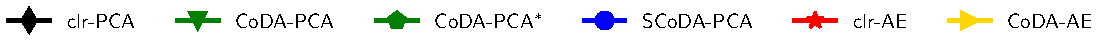
\includegraphics[width=\textwidth]{legend_ext}\\%
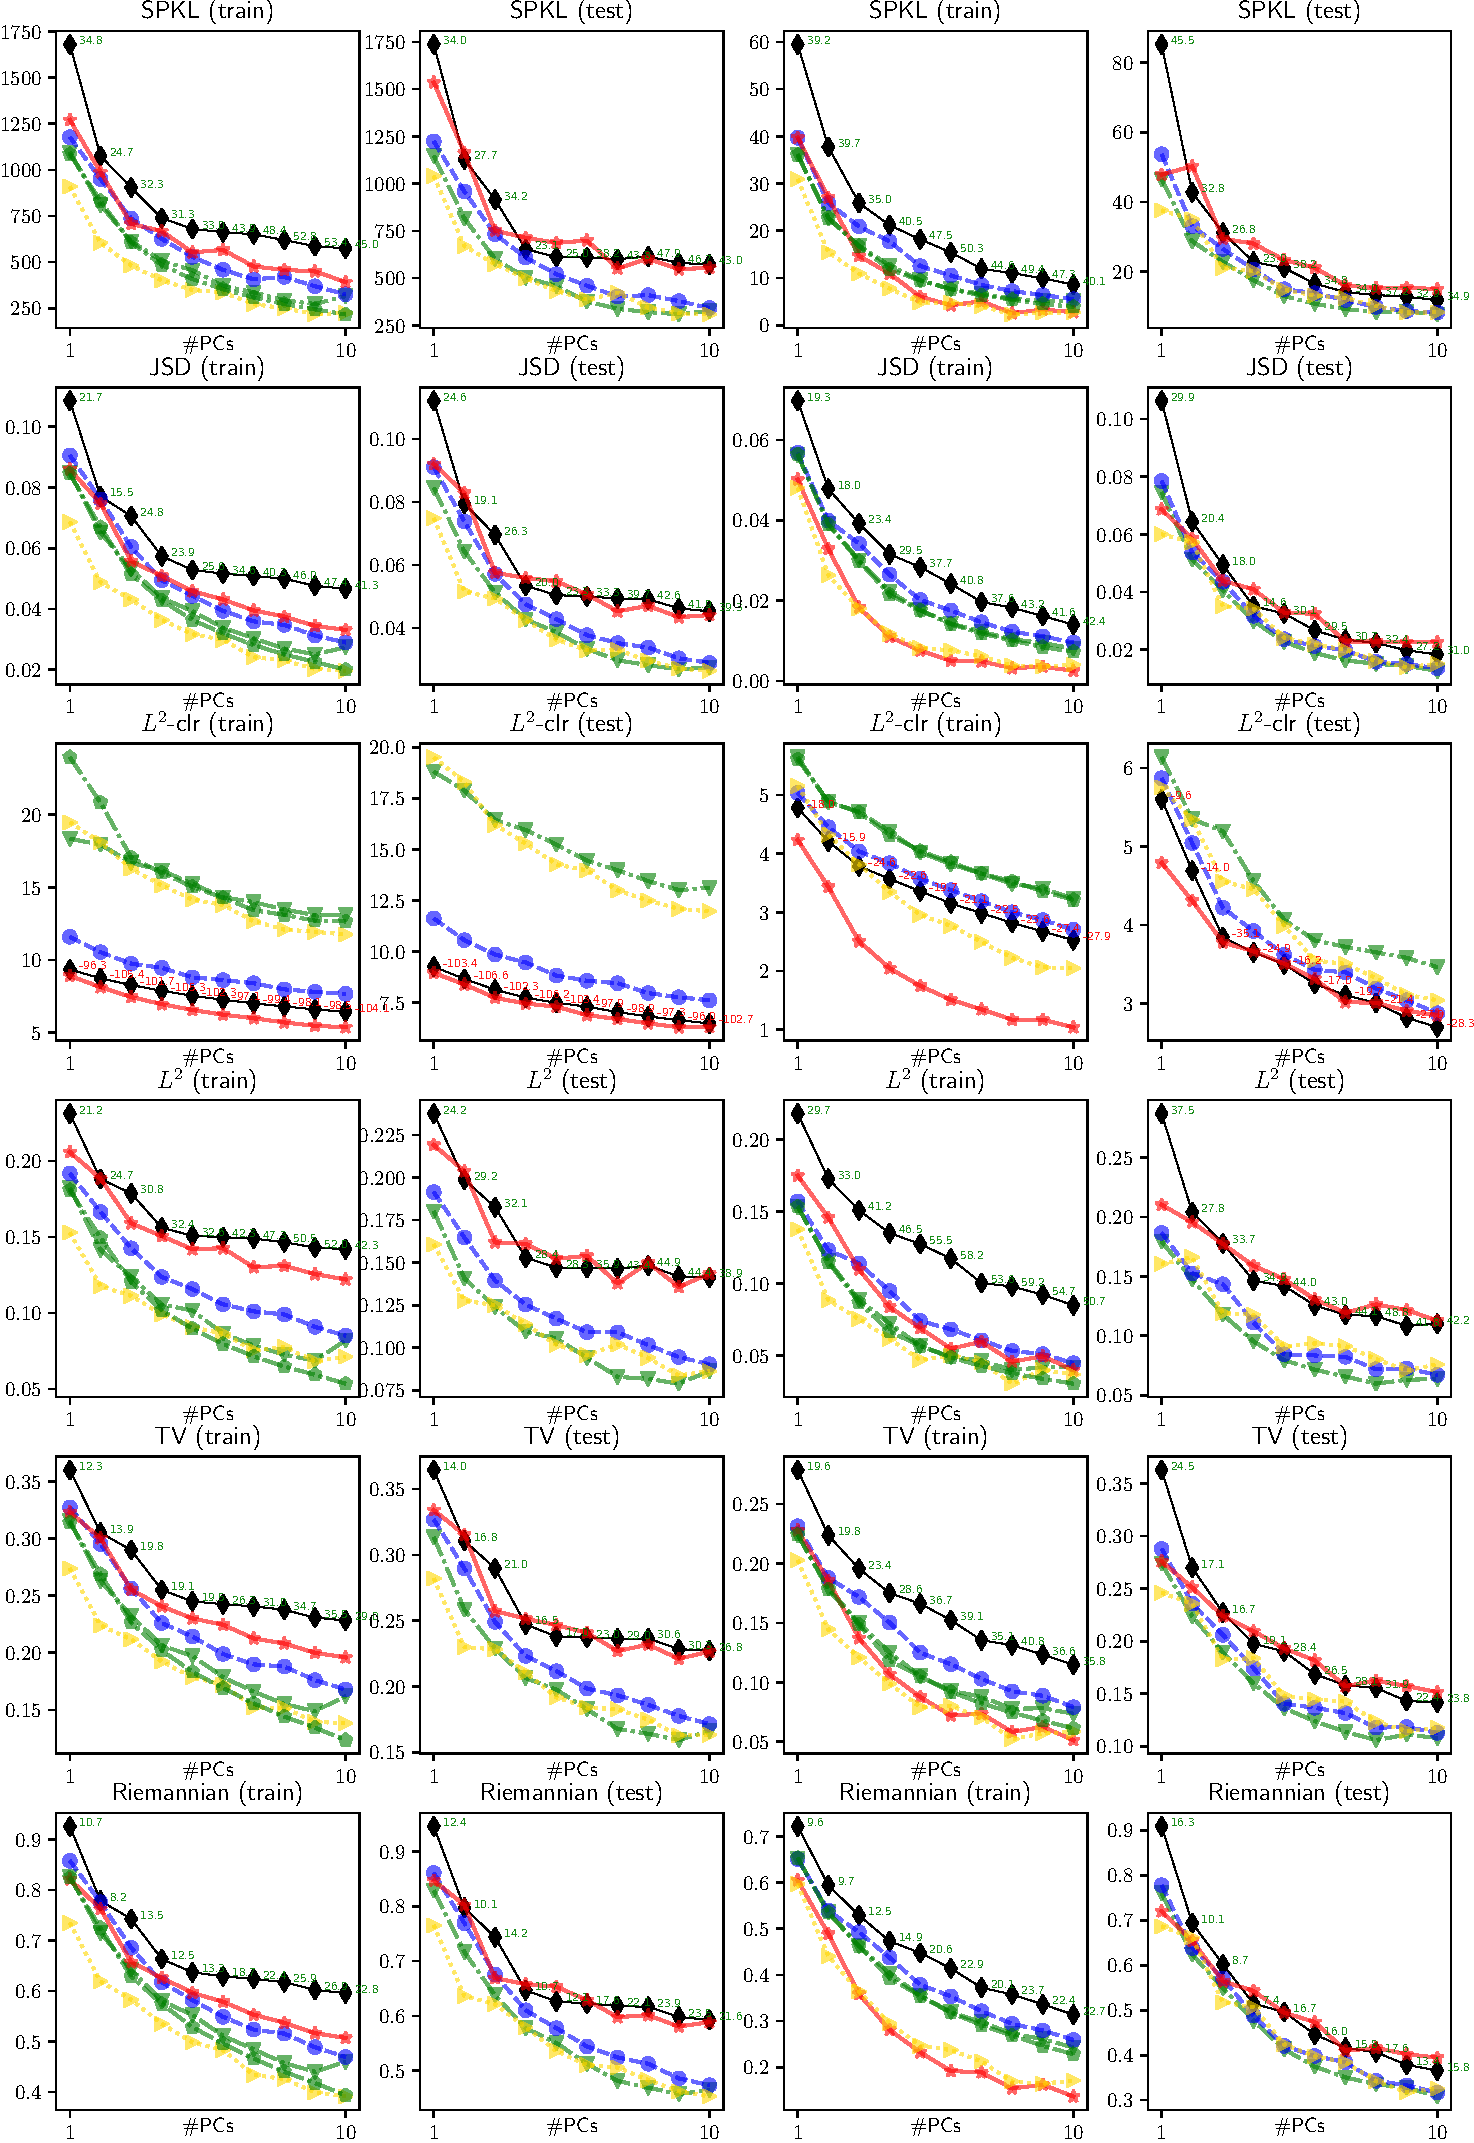
\includegraphics[width=\textwidth]{fullcurves}%
\caption{Training and testing errors measured by different distances
against the number of principal components.
The columns, from left to right, show training errors (Atlas),
corresponding testing errors, training errors (diet swap) and corresponding test errors.\label{fig:fullresult}}
\end{figure}




%\bibliographystyle{plain}
%\bibliography{bibgen}

%\end{document}
